%==============================================================
%  Figura 6.13 - Disposizione in serie di sottosistemi per la
%  realizzazione di una funzione di sicurezza
%  Adattamento in italiano della Figura 6.13 dell'IFA Report 2/2017
%
%  A differenza delle altre figure del capitolo, qui il disegno non e'
%  stato ricostruito a mano: i simboli (cilindro, barriera, valvola,
%  schemi a blocchi) sono troppi e troppo minuti. Il blocco "geometria"
%  qui sotto e' la conversione automatica dei 249 tracciati vettoriali
%  della pagina 72 di rep0217e.pdf, che non contengono testo; le
%  diciture italiane sono poi collocate a mano in fondo al file, sulle
%  posizioni misurate nell'originale.
%  Per rigenerare la geometria occorre riconvertire la pagina: il
%  blocco non va modificato a mano.
%
%  Sistema di riferimento: l'origine e' l'angolo in basso a sinistra
%  della cornice; l'asse y e' rivolto verso l'alto; una unita' e' un
%  punto PostScript del disegno originale.
%==============================================================
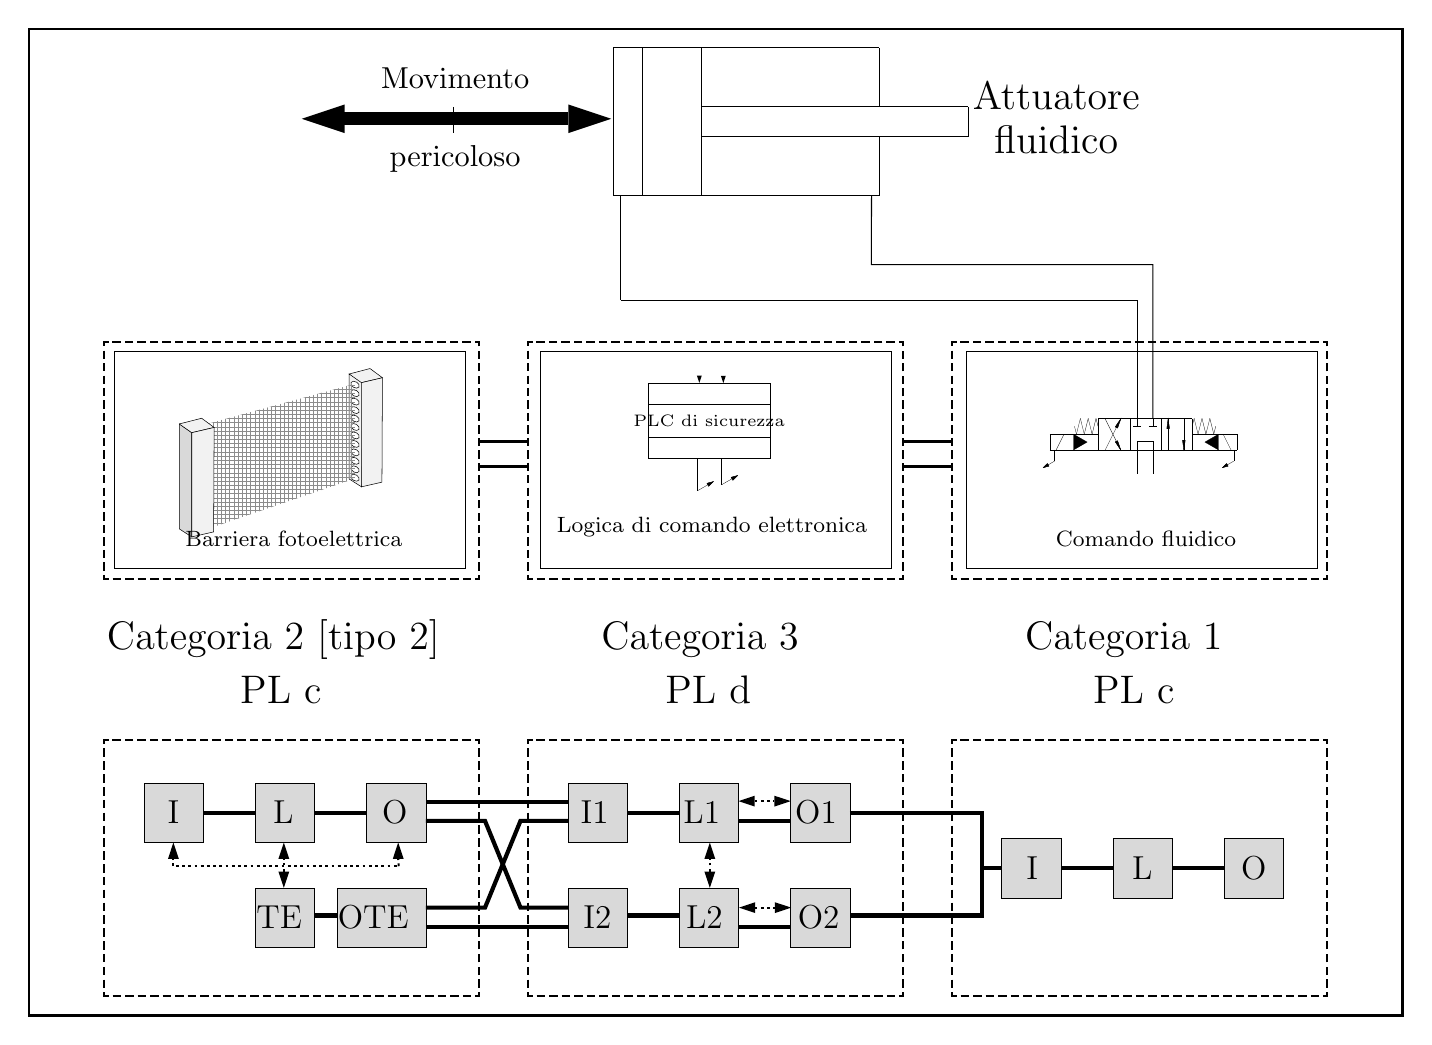
\begin{tikzpicture}[
  x=0.035cm, y=0.035cm,
  piccolo/.style={font=\fontsize{8.2}{9.5}\selectfont},
  medio/.style={font=\fontsize{11}{13}\selectfont},
  grande/.style={font=\fontsize{13.7}{16}\selectfont},
  siglablocco/.style={font=\fontsize{12.6}{15}\selectfont}
]

\setstretch{1}

% ============ geometria (conversione automatica, non modificare) ============
\filldraw[fill=white, draw=black, line width=0.19pt] (340.02,240.97) -- (467.39,240.97) -- (467.39,162.26) -- (340.02,162.26) -- cycle;
\filldraw[fill=white, draw=black, line width=0.19pt] (185.46,240.97) -- (312.83,240.97) -- (312.83,162.26) -- (185.46,162.26) -- cycle;
\filldraw[fill=white, draw=black, line width=0.19pt] (30.91,240.97) -- (158.27,240.97) -- (158.27,162.26) -- (30.91,162.26) -- cycle;
\fill[fill=black] (114.49,320.22) -- (98.95,325.4) -- (114.49,330.58) -- cycle;
\fill[fill=black] (195.68,330.58) -- (211.22,325.4) -- (195.68,320.22) -- cycle;
\draw[draw=black, line width=0.75pt] (335.01,159.95) -- (335.01,158.44) -- (336.53,158.44);
\draw[draw=black, line width=0.75pt, dash pattern=on 3.01pt off 1.51pt] (338.03,158.44) -- (468.69,158.44);
\draw[draw=black, line width=0.75pt] (469.45,158.44) -- (470.96,158.44) -- (470.96,159.95);
\draw[draw=black, line width=0.75pt, dash pattern=on 3.00pt off 1.50pt] (470.96,161.46) -- (470.96,242.04);
\draw[draw=black, line width=0.75pt] (470.96,242.79) -- (470.96,244.31) -- (469.45,244.31);
\draw[draw=black, line width=0.75pt, dash pattern=on 3.01pt off 1.51pt] (467.94,244.31) -- (337.28,244.31);
\draw[draw=black, line width=0.75pt] (336.53,244.31) -- (335.01,244.31) -- (335.01,242.79);
\draw[draw=black, line width=0.75pt, dash pattern=on 3.00pt off 1.50pt] (335.01,241.29) -- (335.01,160.71);
\draw[draw=black, line width=0.75pt] (181.17,159.95) -- (181.17,158.44) -- (182.68,158.44);
\draw[draw=black, line width=0.75pt, dash pattern=on 3.01pt off 1.51pt] (184.19,158.44) -- (314.85,158.44);
\draw[draw=black, line width=0.75pt] (315.6,158.44) -- (317.12,158.44) -- (317.12,159.95);
\draw[draw=black, line width=0.75pt, dash pattern=on 3.00pt off 1.50pt] (317.12,161.46) -- (317.12,242.04);
\draw[draw=black, line width=0.75pt] (317.12,242.79) -- (317.12,244.31) -- (315.61,244.31);
\draw[draw=black, line width=0.75pt, dash pattern=on 3.01pt off 1.51pt] (314.1,244.31) -- (183.44,244.31);
\draw[draw=black, line width=0.75pt] (182.69,244.31) -- (181.17,244.31) -- (181.17,242.79);
\draw[draw=black, line width=0.75pt, dash pattern=on 3.00pt off 1.50pt] (181.17,241.29) -- (181.17,160.71);
\draw[draw=black, line width=0.75pt] (27.33,159.95) -- (27.33,158.44) -- (28.84,158.44);
\draw[draw=black, line width=0.75pt, dash pattern=on 3.01pt off 1.51pt] (30.35,158.44) -- (161.01,158.44);
\draw[draw=black, line width=0.75pt] (161.76,158.44) -- (163.28,158.44) -- (163.28,159.95);
\draw[draw=black, line width=0.75pt, dash pattern=on 3.00pt off 1.50pt] (163.28,161.46) -- (163.28,242.04);
\draw[draw=black, line width=0.75pt] (163.28,242.79) -- (163.28,244.31) -- (161.77,244.31);
\draw[draw=black, line width=0.75pt, dash pattern=on 3.01pt off 1.51pt] (160.26,244.31) -- (29.6,244.31);
\draw[draw=black, line width=0.75pt] (28.85,244.31) -- (27.33,244.31) -- (27.33,242.79);
\draw[draw=black, line width=0.75pt, dash pattern=on 3.00pt off 1.50pt] (27.33,241.29) -- (27.33,160.71);
\draw[draw=black, line width=1.13pt] (316.83,208.41) -- (334.73,208.41);
\draw[draw=black, line width=1.13pt] (317.12,199.11) -- (335.01,199.11);
\draw[draw=black, line width=1.13pt] (162.99,208.41) -- (180.89,208.41);
\draw[draw=black, line width=1.13pt] (163.28,199.11) -- (181.17,199.11);
\draw[draw=black, line width=0.75pt] (27.33,8.5) -- (27.33,6.99) -- (28.84,6.99);
\draw[draw=black, line width=0.75pt, dash pattern=on 3.01pt off 1.51pt] (30.35,6.99) -- (161.01,6.99);
\draw[draw=black, line width=0.75pt] (161.76,6.99) -- (163.28,6.99) -- (163.28,8.5);
\draw[draw=black, line width=0.75pt, dash pattern=on 3.09pt off 1.55pt] (163.28,10.05) -- (163.28,97.72);
\draw[draw=black, line width=0.75pt] (163.28,98.49) -- (163.28,100.01) -- (161.77,100.01);
\draw[draw=black, line width=0.75pt, dash pattern=on 3.01pt off 1.51pt] (160.26,100.01) -- (29.6,100.01);
\draw[draw=black, line width=0.75pt] (28.85,100.01) -- (27.33,100.01) -- (27.33,98.49);
\draw[draw=black, line width=0.75pt, dash pattern=on 3.09pt off 1.55pt] (27.33,96.94) -- (27.33,9.28);
\filldraw[fill=black!15, draw=black, line width=0.19pt] (82.07,46.34) -- (103.53,46.34) -- (103.53,24.88) -- (82.07,24.88) -- cycle;
\draw[draw=black, line width=1.51pt] (63.11,73.53) -- (122.49,73.53);
\filldraw[fill=black!15, draw=black, line width=0.19pt] (41.64,84.26) -- (63.11,84.26) -- (63.11,62.8) -- (41.64,62.8) -- cycle;
\filldraw[fill=black!15, draw=black, line width=0.19pt] (82.07,84.26) -- (103.53,84.26) -- (103.53,62.8) -- (82.07,62.8) -- cycle;
\fill[fill=black!15] (122.5,84.26) -- (143.96,84.26) -- (143.96,62.8) -- (122.5,62.8) -- cycle;
\draw[draw=black, line width=0.19pt] (122.49,84.26) -- (143.96,84.26) -- (143.96,62.8) -- (122.49,62.8) -- cycle;
\fill[fill=black!15] (111.76,46.34) -- (143.96,46.34) -- (143.96,24.88) -- (111.76,24.88) -- cycle;
\draw[draw=black, line width=0.19pt] (111.76,46.34) -- (143.96,46.34) -- (143.96,24.88) -- (111.76,24.88) -- cycle;
\draw[draw=black, line width=0.75pt] (181.17,8.5) -- (181.17,6.99) -- (182.68,6.99);
\draw[draw=black, line width=0.75pt, dash pattern=on 3.01pt off 1.51pt] (184.19,6.99) -- (314.85,6.99);
\draw[draw=black, line width=0.75pt] (315.6,6.99) -- (317.12,6.99) -- (317.12,8.5);
\draw[draw=black, line width=0.75pt, dash pattern=on 3.09pt off 1.55pt] (317.12,10.05) -- (317.12,97.72);
\draw[draw=black, line width=0.75pt] (317.12,98.49) -- (317.12,100.01) -- (315.61,100.01);
\draw[draw=black, line width=0.75pt, dash pattern=on 3.01pt off 1.51pt] (314.1,100.01) -- (183.44,100.01);
\draw[draw=black, line width=0.75pt] (182.69,100.01) -- (181.17,100.01) -- (181.17,98.49);
\draw[draw=black, line width=0.75pt, dash pattern=on 3.09pt off 1.55pt] (181.17,96.94) -- (181.17,9.28);
\filldraw[fill=black!15, draw=black, line width=0.19pt] (195.48,84.26) -- (216.95,84.26) -- (216.95,62.8) -- (195.48,62.8) -- cycle;
\filldraw[fill=black!15, draw=black, line width=0.19pt] (235.91,84.26) -- (257.37,84.26) -- (257.37,62.8) -- (235.91,62.8) -- cycle;
\fill[fill=black!15] (276.33,84.26) -- (297.8,84.26) -- (297.8,62.8) -- (276.33,62.8) -- cycle;
\draw[draw=black, line width=0.19pt] (276.34,84.26) -- (297.8,84.26) -- (297.8,62.8) -- (276.34,62.8) -- cycle;
\draw[draw=black, line width=0.75pt] (335.01,8.5) -- (335.01,6.99) -- (336.53,6.99);
\draw[draw=black, line width=0.75pt, dash pattern=on 3.01pt off 1.51pt] (338.03,6.99) -- (468.69,6.99);
\draw[draw=black, line width=0.75pt] (469.45,6.99) -- (470.96,6.99) -- (470.96,8.5);
\draw[draw=black, line width=0.75pt, dash pattern=on 3.09pt off 1.55pt] (470.96,10.05) -- (470.96,97.72);
\draw[draw=black, line width=0.75pt] (470.96,98.49) -- (470.96,100.01) -- (469.45,100.01);
\draw[draw=black, line width=0.75pt, dash pattern=on 3.01pt off 1.51pt] (467.94,100.01) -- (337.28,100.01);
\draw[draw=black, line width=0.75pt] (336.53,100.01) -- (335.01,100.01) -- (335.01,98.49);
\draw[draw=black, line width=0.75pt, dash pattern=on 3.09pt off 1.55pt] (335.01,96.94) -- (335.01,9.28);
\draw[draw=black, line width=1.51pt] (345.39,53.5) -- (433.75,53.5);
\filldraw[fill=black!15, draw=black, line width=0.19pt] (352.9,64.23) -- (374.36,64.23) -- (374.36,42.76) -- (352.9,42.76) -- cycle;
\filldraw[fill=black!15, draw=black, line width=0.19pt] (393.33,64.23) -- (414.79,64.23) -- (414.79,42.76) -- (393.33,42.76) -- cycle;
\filldraw[fill=black!15, draw=black, line width=0.19pt] (433.75,64.23) -- (455.22,64.23) -- (455.22,42.76) -- (433.75,42.76) -- cycle;
\filldraw[fill=black!15, draw=black, line width=0.19pt] (195.48,46.34) -- (216.95,46.34) -- (216.95,24.88) -- (195.48,24.88) -- cycle;
\filldraw[fill=black!15, draw=black, line width=0.19pt] (235.91,46.34) -- (257.37,46.34) -- (257.37,24.88) -- (235.91,24.88) -- cycle;
\fill[fill=black!15] (276.33,46.34) -- (297.8,46.34) -- (297.8,24.88) -- (276.33,24.88) -- cycle;
\draw[draw=black, line width=0.19pt] (276.34,46.34) -- (297.8,46.34) -- (297.8,24.88) -- (276.34,24.88) -- cycle;
\draw[draw=black, line width=1.51pt] (103.53,36.32) -- (111.76,36.32);
\draw[draw=black, line width=1.51pt] (143.96,32.03) -- (195.48,32.03);
\draw[draw=black, line width=1.51pt] (143.96,39.19) -- (165.43,39.19) -- (178.31,70.67) -- (195.48,70.67);
\draw[draw=black, line width=1.51pt] (143.96,70.67) -- (165.43,70.67) -- (178.31,39.19) -- (195.48,39.19);
\draw[draw=black, line width=1.51pt] (143.96,77.4) -- (195.48,77.4);
\draw[draw=black, line width=1.51pt] (216.95,73.53) -- (235.91,73.53);
\draw[draw=black, line width=1.51pt] (216.95,36.32) -- (235.91,36.32);
\draw[draw=black, line width=1.51pt] (257.37,70.67) -- (276.34,70.67);
\fill[fill=black] (263.28,75.86) -- (257.38,77.83) -- (263.28,79.79) -- cycle;
\fill[fill=black] (270.43,79.79) -- (276.34,77.83) -- (270.43,75.85) -- cycle;
\draw[draw=black, line width=1.51pt] (257.55,32.03) -- (276.51,32.03);
\fill[fill=black] (263.46,37.22) -- (257.55,39.19) -- (263.46,41.15) -- cycle;
\fill[fill=black] (270.61,41.15) -- (276.51,39.19) -- (270.61,37.22) -- cycle;
\draw[draw=black, line width=1.51pt] (297.8,73.53) -- (345.74,73.53) -- (345.74,36.33) -- (297.8,36.33);
\fill[fill=black] (90.48,56.89) -- (92.44,62.8) -- (94.41,56.89) -- cycle;
\fill[fill=black] (94.41,52.25) -- (92.44,46.34) -- (90.48,52.25) -- cycle;
\fill[fill=black] (50.41,56.89) -- (52.37,62.8) -- (54.34,56.89) -- cycle;
\fill[fill=black] (131.98,56.89) -- (133.94,62.8) -- (135.91,56.89) -- cycle;
\fill[fill=black] (245.03,56.89) -- (247,62.8) -- (248.97,56.89) -- cycle;
\fill[fill=black] (248.97,52.25) -- (247,46.34) -- (245.03,52.25) -- cycle;
\draw[draw=black, line width=0.10pt] (402.03,196.6) -- (402.03,208.54);
\draw[draw=black, line width=0.10pt] (407.77,213.8) -- (407.77,216.65);
\draw[draw=black, line width=0.10pt] (400.62,213.78) -- (403.47,213.78);
\draw[draw=black, line width=0.10pt] (402.08,216.65) -- (402.08,213.8);
\draw[draw=black, line width=0.10pt] (407.77,196.6) -- (407.77,208.55);
\draw[draw=black, line width=0.10pt] (422.01,205.26) -- (410.62,205.26);
\draw[draw=black, line width=0.10pt] (422.01,216.65) -- (422.01,205.26);
\draw[draw=black, line width=0.10pt] (410.62,216.65) -- (422.01,216.65);
\draw[draw=black, line width=0.10pt] (399.23,216.65) -- (410.62,216.65);
\draw[draw=black, line width=0.10pt] (410.62,205.26) -- (399.23,205.26);
\draw[draw=black, line width=0.10pt] (387.84,205.26) -- (387.84,216.65);
\draw[draw=black, line width=0.10pt] (387.84,216.65) -- (399.23,216.65);
\draw[draw=black, line width=0.10pt] (399.23,205.26) -- (387.84,205.26);
\draw[draw=black, line width=0.10pt] (438.28,210.95) -- (422.01,210.95);
\draw[draw=black, line width=0.10pt] (438.28,205.26) -- (438.28,210.95);
\draw[draw=black, line width=0.10pt] (422.01,205.26) -- (438.28,205.26);
\draw[draw=black, line width=0.10pt] (370.42,210.94) -- (378.96,210.94);
\draw[draw=black, line width=0.10pt] (370.42,205.25) -- (370.42,210.94);
\draw[draw=black, line width=0.10pt] (433.25,210.95) -- (436.09,205.26);
\draw[draw=black, line width=0.10pt] (375.5,210.94) -- (372.65,205.25);
\draw[draw=black, line width=0.10pt] (410.62,205.26) -- (410.62,216.65);
\filldraw[fill=black, draw=black, line width=0.10pt] (431.55,210.94) -- (426.62,208.1) -- (431.55,205.25) -- cycle;
\filldraw[fill=black, draw=black, line width=0.10pt] (378.97,210.94) -- (383.9,208.1) -- (378.97,205.25) -- cycle;
\draw[draw=black, line width=0.10pt] (385.7,210.98) -- (387.12,216.68);
\draw[draw=black, line width=0.10pt] (381.43,216.68) -- (382.85,210.98);
\draw[draw=black, line width=0.10pt] (384.28,216.67) -- (382.85,210.98);
\draw[draw=black, line width=0.10pt] (381.43,216.67) -- (380.01,210.98);
\draw[draw=black, line width=0.10pt] (384.28,216.68) -- (385.7,210.98);
\draw[draw=black, line width=0.10pt] (380.01,210.98) -- (379.3,213.83);
\draw[draw=black, line width=0.10pt] (387.12,216.68) -- (387.84,213.83);
\draw[draw=black, line width=0.10pt] (426.99,210.98) -- (428.42,216.68);
\draw[draw=black, line width=0.10pt] (426.99,210.98) -- (425.57,216.68);
\draw[draw=black, line width=0.10pt] (428.42,216.68) -- (429.84,210.98);
\draw[draw=black, line width=0.10pt] (424.14,210.98) -- (422.72,216.68);
\draw[draw=black, line width=0.10pt] (424.14,210.98) -- (425.57,216.68);
\draw[draw=black, line width=0.10pt] (422.72,216.67) -- (422.01,213.83);
\draw[draw=black, line width=0.10pt] (429.84,210.98) -- (430.55,213.83);
\draw[draw=black, line width=0.10pt] (387.83,210.94) -- (371.56,210.94);
\draw[draw=black, line width=0.10pt] (387.84,205.25) -- (387.84,210.94);
\draw[draw=black, line width=0.10pt] (370.42,205.25) -- (387.84,205.25);
\draw[draw=black, line width=0.10pt] (268.95,229.57) -- (224.58,229.57) -- (224.58,222.04) -- (268.95,222.04) -- cycle;
\draw[draw=black, line width=0.10pt] (268.95,222.04) -- (224.58,222.04) -- (224.58,209.73) -- (268.95,209.73) -- cycle;
\draw[draw=black, line width=0.10pt] (251.23,202.3) -- (251.23,192.59);
\draw[draw=black, line width=0.10pt] (257.07,195.96) -- (251.23,192.59);
\filldraw[fill=black, draw=black, line width=0.10pt] (257.06,195.96) -- (254.73,195.33) -- (255.35,194.25) -- cycle;
\draw[draw=black, line width=0.10pt] (254.73,195.33) -- (257.07,195.96);
\draw[draw=black, line width=0.10pt] (255.35,194.25) -- (257.07,195.96);
\draw[draw=black, line width=0.10pt] (254.73,195.33) -- (255.35,194.25);
\draw[draw=black, line width=0.10pt] (242.47,202.3) -- (242.47,190.4);
\draw[draw=black, line width=0.10pt] (248.31,193.77) -- (242.47,190.4);
\filldraw[fill=black, draw=black, line width=0.10pt] (248.31,193.77) -- (245.97,193.15) -- (246.6,192.06) -- cycle;
\draw[draw=black, line width=0.10pt] (245.97,193.15) -- (248.31,193.77);
\draw[draw=black, line width=0.10pt] (246.6,192.06) -- (248.31,193.77);
\draw[draw=black, line width=0.10pt] (245.97,193.15) -- (246.6,192.06);
\draw[draw=black, line width=0.10pt] (224.58,209.91) -- (224.58,202.36) -- (268.95,202.36) -- (268.95,209.9);
\fill[fill=black] (252.79,232.14) -- (251.91,229.49) -- (251.03,232.14) -- cycle;
\fill[fill=black] (244.07,232.22) -- (243.18,229.58) -- (242.3,232.22) -- cycle;
\draw[draw=black, line width=0.10pt] (372.07,205.27) -- (372.07,201.18);
\draw[draw=black, line width=0.10pt] (367.99,198.83) -- (372.07,201.18);
\filldraw[fill=black, draw=black, line width=0.10pt] (367.99,198.83) -- (370.03,199.37) -- (369.49,200.32) -- cycle;
\draw[draw=black, line width=0.10pt] (370.03,199.37) -- (367.99,198.83);
\draw[draw=black, line width=0.10pt] (369.48,200.32) -- (367.99,198.83);
\draw[draw=black, line width=0.10pt] (370.03,199.37) -- (369.48,200.32);
\draw[draw=black, line width=0.10pt] (437.08,205.27) -- (437.08,201.18);
\draw[draw=black, line width=0.10pt] (433,198.83) -- (437.08,201.18);
\filldraw[fill=black, draw=black, line width=0.10pt] (433,198.83) -- (435.04,199.37) -- (434.49,200.32) -- cycle;
\draw[draw=black, line width=0.10pt] (435.04,199.37) -- (433,198.83);
\draw[draw=black, line width=0.10pt] (434.49,200.32) -- (433,198.83);
\draw[draw=black, line width=0.10pt] (435.04,199.37) -- (434.49,200.32);
\filldraw[fill=black!15, draw=black, line width=0.19pt] (59.03,173.7) -- (59.03,211.51) -- (54.52,214.68) -- (54.52,176.6) -- cycle;
\filldraw[fill=black!5, draw=black, line width=0.19pt] (128.22,231.44) -- (120.1,229.54) -- (116.13,232.79) -- (123.71,234.78) -- cycle;
\filldraw[fill=black!5, draw=black, line width=0.19pt] (128.22,231.44) -- (120.1,229.54) -- (120.63,191.87) -- (128.04,193.55) -- cycle;
\filldraw[fill=black!5, draw=black, line width=0.19pt] (120.63,191.87) -- (120.64,229.63) -- (116.13,232.8) -- (116.13,194.72) -- cycle;
\fill[fill=white] (118.82,229.85) .. controls (119.61,229.39) and (120.01,228.6) .. (119.71,228.08) .. controls (119.41,227.57) and (118.53,227.52) .. (117.73,227.97) .. controls (116.94,228.44) and (116.54,229.22) .. (116.84,229.74) .. controls (117.14,230.26) and (118.02,230.31) .. (118.82,229.85);
\draw[draw=black, line width=0.19pt] (118.82,229.85) .. controls (119.61,229.39) and (120.01,228.6) .. (119.71,228.08) .. controls (119.41,227.57) and (118.53,227.52) .. (117.73,227.97) .. controls (116.94,228.44) and (116.54,229.22) .. (116.84,229.74) .. controls (117.14,230.26) and (118.02,230.31) .. (118.82,229.85) -- cycle;
\fill[fill=white] (118.82,226.78) .. controls (119.61,226.32) and (120.01,225.53) .. (119.71,225.02) .. controls (119.41,224.5) and (118.53,224.45) .. (117.73,224.91) .. controls (116.94,225.36) and (116.54,226.16) .. (116.84,226.67) .. controls (117.14,227.19) and (118.02,227.24) .. (118.82,226.78);
\draw[draw=black, line width=0.19pt] (118.82,226.78) .. controls (119.61,226.32) and (120.01,225.53) .. (119.71,225.02) .. controls (119.41,224.5) and (118.53,224.45) .. (117.73,224.91) .. controls (116.94,225.36) and (116.54,226.16) .. (116.84,226.67) .. controls (117.14,227.19) and (118.02,227.24) .. (118.82,226.78) -- cycle;
\fill[fill=white] (118.82,223.71) .. controls (119.61,223.26) and (120.01,222.46) .. (119.71,221.95) .. controls (119.41,221.43) and (118.53,221.38) .. (117.73,221.84) .. controls (116.94,222.3) and (116.54,223.09) .. (116.84,223.6) .. controls (117.14,224.12) and (118.02,224.17) .. (118.82,223.71);
\draw[draw=black, line width=0.19pt] (118.82,223.71) .. controls (119.61,223.26) and (120.01,222.46) .. (119.71,221.95) .. controls (119.41,221.43) and (118.53,221.38) .. (117.73,221.84) .. controls (116.94,222.3) and (116.54,223.09) .. (116.84,223.6) .. controls (117.14,224.12) and (118.02,224.17) .. (118.82,223.71) -- cycle;
\fill[fill=white] (118.82,220.65) .. controls (119.61,220.19) and (120.01,219.4) .. (119.71,218.88) .. controls (119.41,218.36) and (118.53,218.31) .. (117.73,218.77) .. controls (116.94,219.23) and (116.54,220.02) .. (116.84,220.54) .. controls (117.14,221.05) and (118.02,221.1) .. (118.82,220.65);
\draw[draw=black, line width=0.19pt] (118.82,220.65) .. controls (119.61,220.19) and (120.01,219.4) .. (119.71,218.88) .. controls (119.41,218.36) and (118.53,218.31) .. (117.73,218.77) .. controls (116.94,219.23) and (116.54,220.02) .. (116.84,220.54) .. controls (117.14,221.05) and (118.02,221.1) .. (118.82,220.65) -- cycle;
\fill[fill=white] (118.82,217.58) .. controls (119.61,217.12) and (120.01,216.33) .. (119.71,215.81) .. controls (119.41,215.29) and (118.53,215.25) .. (117.73,215.7) .. controls (116.94,216.16) and (116.54,216.95) .. (116.84,217.47) .. controls (117.14,217.99) and (118.02,218.03) .. (118.82,217.58);
\draw[draw=black, line width=0.19pt] (118.82,217.58) .. controls (119.61,217.12) and (120.01,216.33) .. (119.71,215.81) .. controls (119.41,215.29) and (118.53,215.25) .. (117.73,215.7) .. controls (116.94,216.16) and (116.54,216.95) .. (116.84,217.47) .. controls (117.14,217.99) and (118.02,218.03) .. (118.82,217.58) -- cycle;
\fill[fill=white] (118.82,214.51) .. controls (119.61,214.05) and (120.01,213.26) .. (119.71,212.74) .. controls (119.41,212.22) and (118.53,212.18) .. (117.73,212.63) .. controls (116.94,213.1) and (116.54,213.88) .. (116.84,214.4) .. controls (117.14,214.92) and (118.02,214.97) .. (118.82,214.51);
\draw[draw=black, line width=0.19pt] (118.82,214.51) .. controls (119.61,214.05) and (120.01,213.26) .. (119.71,212.74) .. controls (119.41,212.22) and (118.53,212.18) .. (117.73,212.63) .. controls (116.94,213.1) and (116.54,213.88) .. (116.84,214.4) .. controls (117.14,214.92) and (118.02,214.97) .. (118.82,214.51) -- cycle;
\fill[fill=white] (118.82,211.44) .. controls (119.61,210.98) and (120.01,210.19) .. (119.71,209.67) .. controls (119.41,209.16) and (118.53,209.11) .. (117.73,209.57) .. controls (116.94,210.02) and (116.54,210.81) .. (116.84,211.33) .. controls (117.14,211.85) and (118.02,211.9) .. (118.82,211.44);
\draw[draw=black, line width=0.19pt] (118.82,211.44) .. controls (119.61,210.98) and (120.01,210.19) .. (119.71,209.67) .. controls (119.41,209.16) and (118.53,209.11) .. (117.73,209.57) .. controls (116.94,210.03) and (116.54,210.81) .. (116.84,211.33) .. controls (117.14,211.85) and (118.02,211.9) .. (118.82,211.44) -- cycle;
\fill[fill=white] (118.82,208.37) .. controls (119.61,207.92) and (120.01,207.12) .. (119.71,206.61) .. controls (119.41,206.09) and (118.53,206.04) .. (117.73,206.5) .. controls (116.94,206.96) and (116.54,207.75) .. (116.84,208.26) .. controls (117.14,208.78) and (118.02,208.83) .. (118.82,208.37);
\draw[draw=black, line width=0.19pt] (118.82,208.37) .. controls (119.61,207.92) and (120.01,207.12) .. (119.71,206.61) .. controls (119.41,206.09) and (118.53,206.04) .. (117.73,206.5) .. controls (116.94,206.96) and (116.54,207.75) .. (116.84,208.26) .. controls (117.14,208.78) and (118.02,208.83) .. (118.82,208.37) -- cycle;
\fill[fill=white] (118.82,205.3) .. controls (119.61,204.85) and (120.01,204.06) .. (119.71,203.54) .. controls (119.41,203.02) and (118.53,202.97) .. (117.73,203.43) .. controls (116.94,203.89) and (116.54,204.68) .. (116.84,205.2) .. controls (117.14,205.71) and (118.02,205.76) .. (118.82,205.3);
\draw[draw=black, line width=0.19pt] (118.82,205.3) .. controls (119.61,204.85) and (120.01,204.06) .. (119.71,203.54) .. controls (119.41,203.02) and (118.53,202.97) .. (117.73,203.43) .. controls (116.94,203.89) and (116.54,204.68) .. (116.84,205.2) .. controls (117.14,205.71) and (118.02,205.76) .. (118.82,205.3) -- cycle;
\fill[fill=white] (118.82,202.24) .. controls (119.61,201.78) and (120.01,200.99) .. (119.71,200.47) .. controls (119.41,199.95) and (118.53,199.9) .. (117.73,200.36) .. controls (116.94,200.82) and (116.54,201.61) .. (116.84,202.13) .. controls (117.14,202.65) and (118.02,202.69) .. (118.82,202.24);
\draw[draw=black, line width=0.19pt] (118.82,202.24) .. controls (119.61,201.78) and (120.01,200.99) .. (119.71,200.47) .. controls (119.41,199.95) and (118.53,199.9) .. (117.73,200.36) .. controls (116.94,200.82) and (116.54,201.61) .. (116.84,202.13) .. controls (117.14,202.65) and (118.02,202.69) .. (118.82,202.24) -- cycle;
\fill[fill=white] (118.82,199.17) .. controls (119.61,198.71) and (120.01,197.92) .. (119.71,197.4) .. controls (119.41,196.88) and (118.53,196.84) .. (117.73,197.29) .. controls (116.94,197.75) and (116.54,198.54) .. (116.84,199.06) .. controls (117.14,199.58) and (118.02,199.62) .. (118.82,199.17);
\draw[draw=black, line width=0.19pt] (118.82,199.17) .. controls (119.61,198.71) and (120.01,197.92) .. (119.71,197.4) .. controls (119.41,196.88) and (118.53,196.84) .. (117.73,197.29) .. controls (116.94,197.75) and (116.54,198.54) .. (116.84,199.06) .. controls (117.14,199.58) and (118.02,199.62) .. (118.82,199.17) -- cycle;
\fill[fill=white] (118.82,196.1) .. controls (119.61,195.64) and (120.01,194.85) .. (119.71,194.33) .. controls (119.41,193.82) and (118.53,193.77) .. (117.73,194.22) .. controls (116.94,194.69) and (116.54,195.47) .. (116.84,195.99) .. controls (117.14,196.51) and (118.02,196.56) .. (118.82,196.1);
\draw[draw=black, line width=0.19pt] (118.82,196.1) .. controls (119.61,195.64) and (120.01,194.85) .. (119.71,194.33) .. controls (119.41,193.82) and (118.53,193.77) .. (117.73,194.22) .. controls (116.94,194.69) and (116.54,195.47) .. (116.84,195.99) .. controls (117.14,196.51) and (118.02,196.56) .. (118.82,196.1) -- cycle;
% fascio della barriera: nell originale e un riempimento a trama ritagliato
% sul parallelogramma; qui e ricostruito come reticolo dello stesso passo
\begin{scope}
  \clip (65.19,214.85) -- (118.21,229.23) -- (118.21,194.87) -- (66.94,177.31) -- cycle;
  \foreach \i in {0,...,36}{\draw[black!45, line width=0.1pt] ({65.19+1.515*\i},177.31) -- ({65.19+1.515*\i},229.23);}
  \foreach \j in {0,...,35}{\draw[black!45, line width=0.1pt] (65.19,{177.31+1.515*\j}) -- (118.21,{177.31+1.515*\j});}
\end{scope}
\filldraw[fill=black!5, draw=black, line width=0.19pt] (67.15,213.4) -- (59.03,211.5) -- (54.52,214.66) -- (54.52,214.68) -- (62.64,216.74) -- cycle;
\filldraw[fill=black!5, draw=black, line width=0.19pt] (67.15,213.4) -- (59.03,211.51) -- (59.03,173.7) -- (66.97,175.51) -- cycle;
\draw[draw=black, line width=0.38pt] (214.62,286.76) -- (214.62,259.6);
\draw[draw=black, line width=0.38pt] (402.13,259.6) -- (214.62,259.6);
\draw[draw=black, line width=0.38pt] (211.94,351.16) -- (308.53,351.16);
\draw[draw=black, line width=0.38pt] (308.53,351.16) -- (308.53,329.69);
\draw[draw=black, line width=0.38pt] (308.53,318.96) -- (308.53,297.49);
\draw[draw=black, line width=0.38pt] (308.53,297.49) -- (211.94,297.49);
\draw[draw=black, line width=0.38pt] (211.94,297.49) -- (211.94,351.16);
\draw[draw=black, line width=0.38pt] (222.67,351.16) -- (222.67,297.49);
\draw[draw=black, line width=0.38pt] (222.67,297.49) -- (233.41,297.49);
\draw[draw=black, line width=0.38pt] (233.41,297.49) -- (244.14,297.49);
\draw[draw=black, line width=0.38pt] (244.14,297.49) -- (244.14,351.16);
\draw[draw=black, line width=0.38pt] (244.14,351.16) -- (222.67,351.16);
\draw[draw=black, line width=0.38pt] (244.14,329.69) -- (340.74,329.69);
\draw[draw=black, line width=0.38pt] (340.73,329.69) -- (340.73,318.96);
\draw[draw=black, line width=0.38pt] (340.73,318.96) -- (244.14,318.96);
\draw[draw=black, line width=0.38pt] (244.14,324.33) -- (244.14,329.69);
\draw[draw=black, line width=0.38pt] (214.62,297.49) -- (214.62,286.76);
\draw[draw=black, line width=0.38pt] (402.08,216.64) -- (402.08,259.54);
\draw[draw=black, line width=0.38pt] (407.78,216.65) -- (407.78,272.45) -- (305.6,272.45) -- (305.64,286.76) -- (305.67,297.49);
\draw[draw=black, line width=0.38pt] (153.98,329.69) -- (153.98,320.39);
\draw[draw=black, line width=0.10pt] (402.03,208.55) -- (407.77,208.55);
\draw[draw=black, line width=0.10pt] (406.28,213.78) -- (409.12,213.78);
\draw[draw=black, line width=0.10pt] (390.42,216.58) -- (396.12,205.19);
\draw[draw=black, line width=0.10pt] (390.42,205.19) -- (396.12,216.58);
\draw[draw=black, line width=0.10pt] (396.12,205.19) -- (394.11,208.16);
\draw[draw=black, line width=0.10pt] (396.12,205.19) -- (394.94,208.58);
\draw[draw=black, line width=0.10pt] (394.94,208.58) -- (394.1,208.17);
\filldraw[fill=black, draw=black, line width=0.10pt] (396.12,205.19) -- (394.94,208.58) -- (394.1,208.16) -- cycle;
\filldraw[fill=black, draw=black, line width=0.10pt] (396.12,216.58) -- (394.94,213.19) -- (394.1,213.61) -- cycle;
\draw[draw=black, line width=0.10pt] (394.94,213.19) -- (394.1,213.6);
\draw[draw=black, line width=0.10pt] (396.12,216.58) -- (394.94,213.19);
\draw[draw=black, line width=0.10pt] (396.12,216.58) -- (394.1,213.61);
\draw[draw=black, line width=0.10pt] (399.32,205.26) -- (399.32,216.65);
\draw[draw=black, line width=0.10pt] (418.98,216.58) -- (418.98,205.19);
\draw[draw=black, line width=0.10pt] (413.29,216.58) -- (413.29,205.19);
\draw[draw=black, line width=0.10pt] (413.29,216.58) -- (412.82,213.02);
\draw[draw=black, line width=0.10pt] (413.29,216.58) -- (413.76,213.02);
\draw[draw=black, line width=0.10pt] (413.76,213.02) -- (412.82,213.02);
\filldraw[fill=black, draw=black, line width=0.10pt] (413.29,216.58) -- (413.76,213.02) -- (412.82,213.02) -- cycle;
\filldraw[fill=black, draw=black, line width=0.10pt] (418.99,205.19) -- (418.52,208.75) -- (419.46,208.75) -- cycle;
\draw[draw=black, line width=0.10pt] (418.52,208.75) -- (419.46,208.75);
\draw[draw=black, line width=0.10pt] (418.99,205.19) -- (418.52,208.75);
\draw[draw=black, line width=0.10pt] (418.99,205.19) -- (419.46,208.75);
\draw[draw=black, line width=0.74pt, dash pattern=on 1.00pt off 1.25pt] (53.26,54.21) -- (134.11,54.21);
\draw[draw=black, line width=0.74pt, dash pattern=on 1.00pt off 1.25pt] (247,52.25) -- (247,56.89);
\draw[draw=black, line width=0.74pt, dash pattern=on 1.00pt off 1.25pt] (134.11,54.21) -- (133.94,56.89);
\draw[draw=black, line width=0.74pt, dash pattern=on 1.00pt off 1.25pt] (92.44,52.25) -- (92.44,56.89);
\draw[draw=black, line width=0.74pt, dash pattern=on 1.00pt off 1.25pt] (52.37,54.21) -- (52.37,56.89);
\draw[draw=black, line width=0.74pt, dash pattern=on 1.00pt off 1.25pt] (263.28,77.83) -- (270.43,77.83);
\draw[draw=black, line width=0.74pt, dash pattern=on 1.00pt off 1.25pt] (263.28,39.19) -- (270.61,39.19);
\draw[draw=black, line width=4.78pt] (113.59,325.4) -- (195.69,325.4);
\draw[draw=black, line width=0.99pt] (-0,-0) -- (498.29,-0) -- (498.29,357.96) -- (-0,357.96) -- cycle;

% ============ diciture italiane (collocate a mano) ============
% movimento pericoloso dell'attuatore
\node[medio] at (154.62,340.10) {Movimento};
\node[medio] at (154.57,310.73) {pericoloso};
\node[grande, align=center] at (372.70,325.60) {Attuatore\\fluidico};

% sottosistemi
% il riquadro del PLC e largo 44,4 unita: a corpo 8,2 la dicitura italiana
% non ci sta, quindi qui scende a 6
\node[font=\fontsize{6}{7}\selectfont] at (246.77,215.89) {PLC di sicurezza};
\node[piccolo] at (96.07,173.12) {Barriera fotoelettrica};
\node[piccolo] at (247.77,177.30) {Logica di comando elettronica};
\node[piccolo] at (405.27,173.12) {Comando fluidico};

% categoria e PL di ciascun sottosistema
\node[grande] at (88.62,136.50) {Categoria 2 [tipo 2]};
\node[grande] at (91.37,118.30) {PL c};
\node[grande] at (243.42,136.50) {Categoria 3};
\node[grande] at (246.42,118.30) {PL d};
\node[grande] at (397.22,136.50) {Categoria 1};
\node[grande] at (400.82,118.30) {PL c};

% sigle degli schemi a blocchi (invariate: sono simboli della norma)
\node[siglablocco] at (52.37,73.65) {I};
\node[siglablocco] at (92.22,73.65) {L};
\node[siglablocco] at (132.72,73.65) {O};
\node[siglablocco] at (205.22,73.65) {I1};
\node[siglablocco] at (244.07,73.65) {L1};
\node[siglablocco] at (285.52,73.65) {O1};
\node[siglablocco] at (90.77,35.68) {TE};
\node[siglablocco] at (124.92,35.68) {OTE};
\node[siglablocco] at (206.17,35.68) {I2};
\node[siglablocco] at (245.02,35.68) {L2};
\node[siglablocco] at (286.47,35.68) {O2};
\node[siglablocco] at (363.97,53.59) {I};
\node[siglablocco] at (403.92,53.59) {L};
\node[siglablocco] at (444.32,53.59) {O};

\end{tikzpicture}
